\documentclass[11pt, oneside]{article} 
\usepackage{geometry}
\geometry{letterpaper} 
\usepackage{graphicx}
	
\usepackage{amssymb}
\usepackage{amsmath}
\usepackage{parskip}
\usepackage{color}
\usepackage{hyperref}

\graphicspath{{/Users/telliott_admin/Dropbox/Tex/png/}}
% \begin{center} 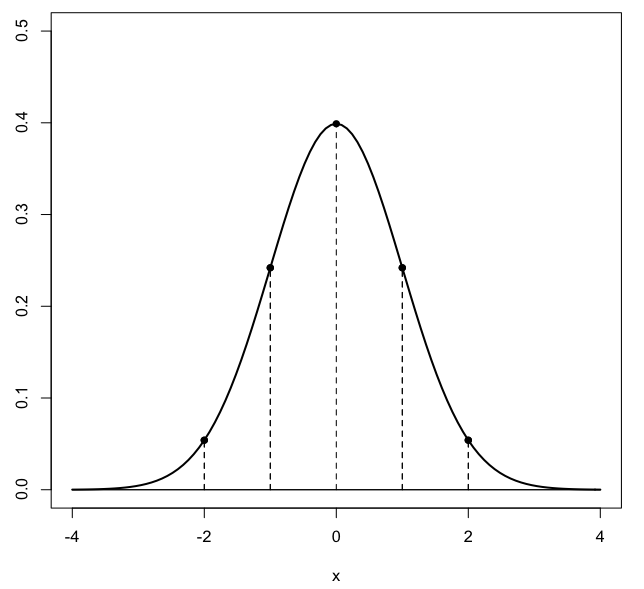
\includegraphics [scale=0.4] {gauss3.png} \end{center}

\title{Limits}
\date{}

\begin{document}
\maketitle
\Large

Consider the graph of a function $f(x)$.  We might choose a power of $x$ similar to $y = x^2$ or $y = x^3 - x$, which affirmatively has two properties that are of interest here:  continuity and differentiability.
\begin{center} 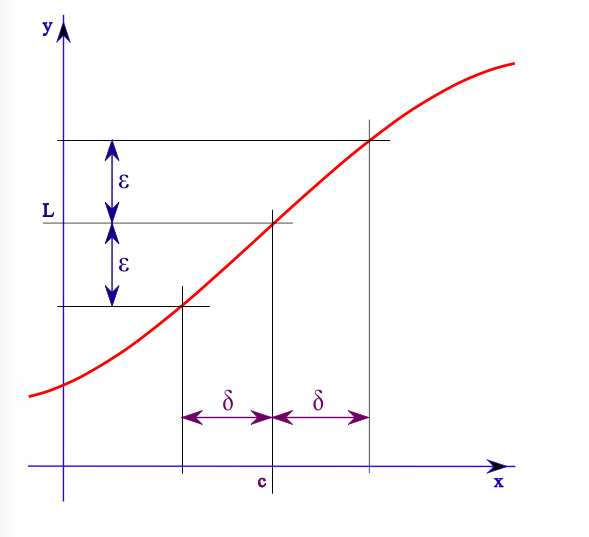
\includegraphics [scale=0.35] {epsilon-delta.png} \end{center}
We focus on the neighborhood of a point on the $x$-axis, $x=c$.

By inspection of the graph we see that the value of $f(x)$ at $c$ is equal to $L$, and furthermore, for points near $c$, the value of $f$ at those points is not too different from $L$.

We would like to say that the \emph{limit} of $f(x)$ as $x$ \emph{approaches} $c$ is equal to $L$.  The idea is that we can make $f(x)$ as close to $L$ as we please, provided we choose $x$ sufficiently close to $c$.

\begin{quote}When the values successively attributed to a variable approach indefinitely to a fixed value, in a manner so as to end by differing from it by as little as one wishes, this last is called the limit of all the others.  ---Cauchy\end{quote}

\begin{center} 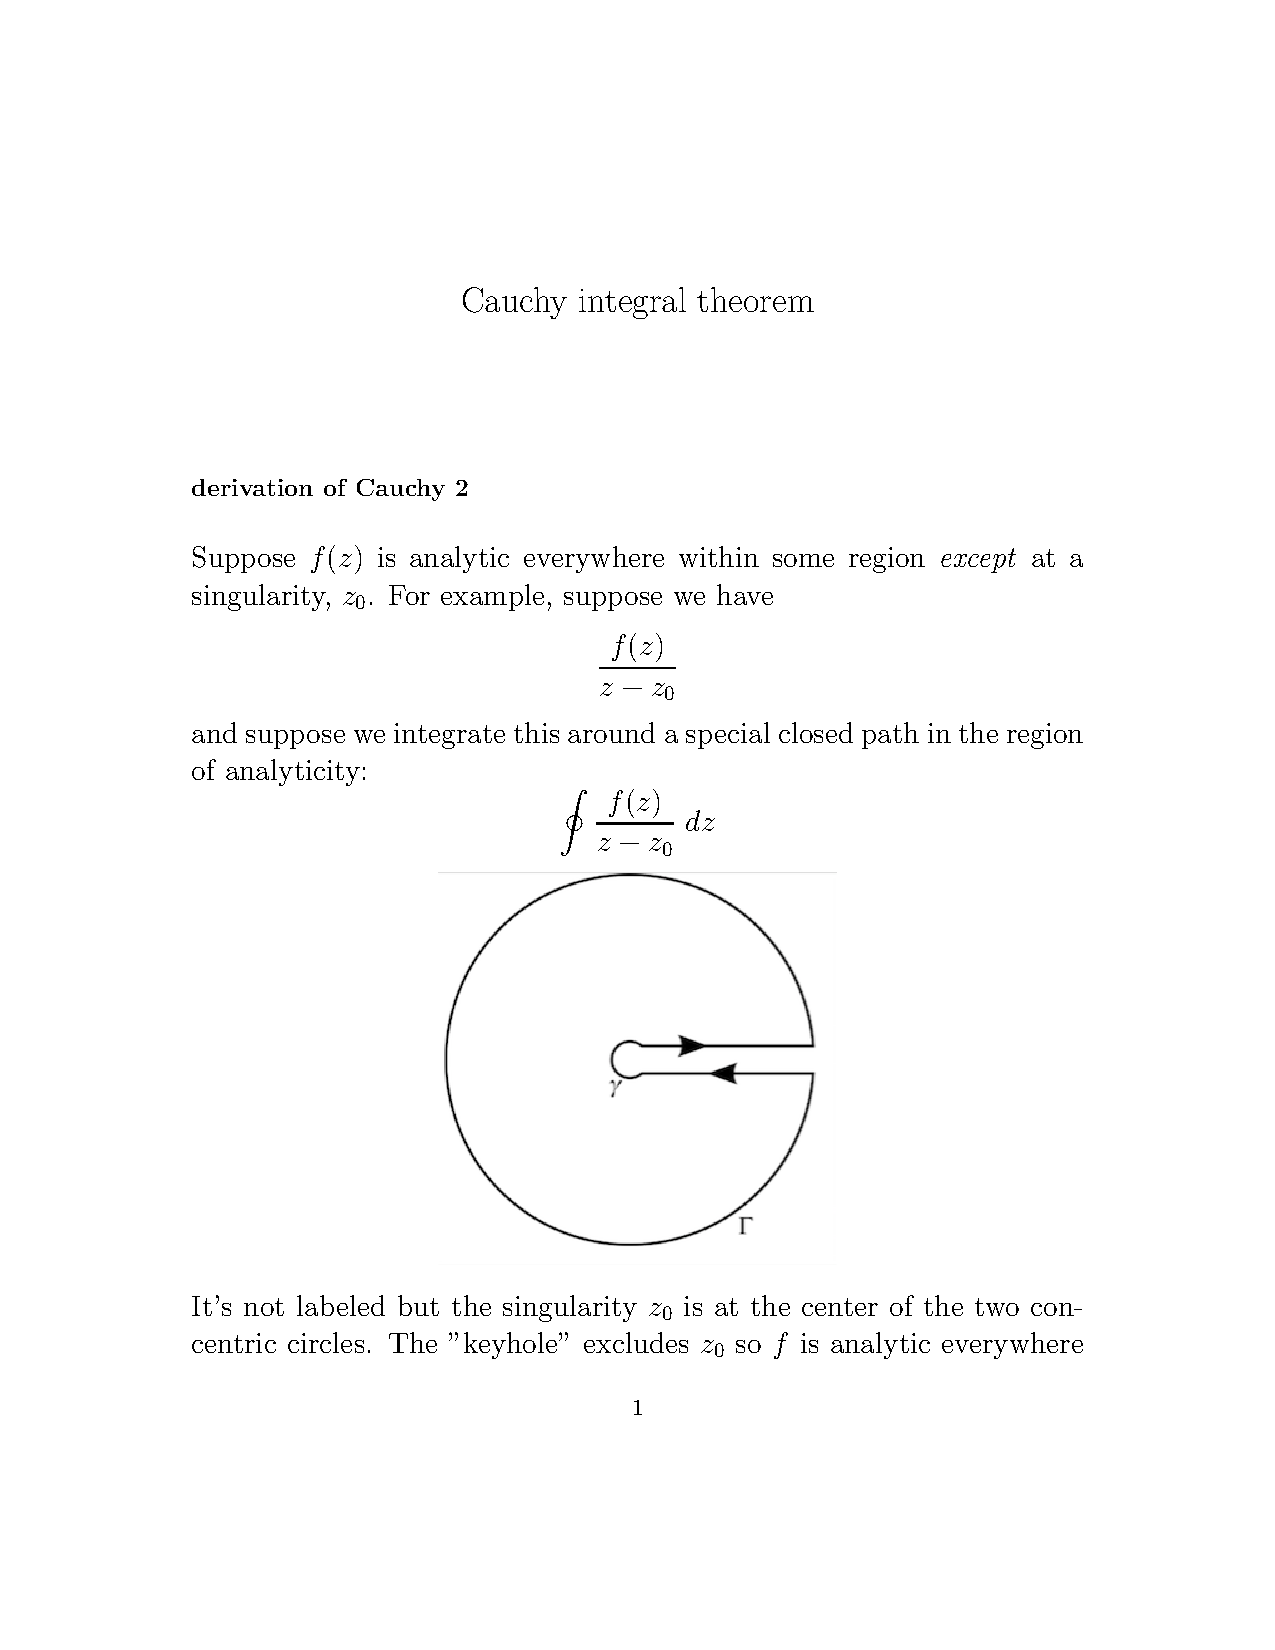
\includegraphics [scale=0.3] {Cauchy} \end{center}

Modern mathematicians don't like that word "approach", which conjures up movement and the involvement of time, and they don't like reasoning from what they see in a graph, in part because no graph can show the whole function for the general case.  Instead we will use an algebraic method from the formal apparatus of calculus.

There are two equivalent approaches, neighborhoods, and epsilon-delta formalism.  Let's look at neighborhoods briefly first.
\subsection*{neighborhoods}

First, an \emph{interval} between two real numbers $a$ and $b$ ($a < b$) contains every real number $a < x < b$.
\[ (a,b) = x \ | \ a < x < b \]
The "$|$" means $x$ "such that" the condition $a < x < b$ holds.

A \emph{closed} interval $[a,b]$ includes the endpoints ($a \le x \le b$), while an \emph{open} interval $(a,b)$ excludes them.  Half-open intervals like $[a,b)$ may be defined, and an interval with $\pm \ \infty$ as an endpoint is always open on that end, for example:  $[a,\infty)$.

Any open interval with a point $p$ as its midpoint is called a \emph{neighborhood} of $p$.  The distance $r$ from $p$ to the boundary of a particular neighborhood may be large or very very small.  We denote a neighborhood of $p$ as $N(p)$.
\[ N(p) = x \ \text{ such that } \ |x-p| < r \].

To say that the limit $f(x) \rightarrow L$ exists, we mean that for every neighborhood $N_1(L)$, there exists some neighborhood $N_2(p)$ such that $f(x) \in N_1(L)$ whenever $x \in N_2(p)$.  

For a limit, we exclude the point $x = p$.  It is not necessary that $f(p) = L$.

The idea of a neighborhood is a nice abstraction to hide the apparatus of modern calculus, which we look at next.
\begin{center} 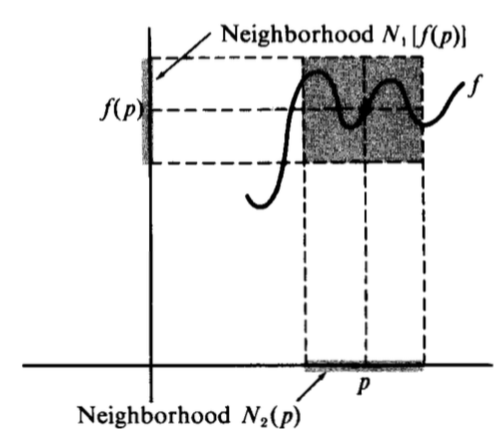
\includegraphics [scale=0.4] {neighborhood.png} \end{center}

\subsection*{epsilon-delta game}
The formal method uses numbers called $\epsilon$ and $\delta$ and is originally due to Bolzano.

We say that, \emph{if} for all points $x$ within a specified distance $\delta$ of $c$, we find that $f(x)$ lies within a specified distance $\epsilon$ from $L$, \emph{then} the limit is $L$.

To do this we must choose $\epsilon$ first.  That's why I call it a game.  Why don't you go first?  Choose $\epsilon$, which provides a constraint on how close to $L$ you want the value of $f(x)$ to be:  you require that  $|f(x) - L| < \epsilon$.  The \emph{distance} from $f(x)$ to $L$ must be less than $\epsilon$.

Now that I know your $\epsilon$, I must try to find a suitable $\delta$.  If I can, then you get another chance, and will presumably choose a smaller $\epsilon$.  

If I can show that it is possible to find a $\delta$ to guarantee that your constraint is satisfied for \emph{all} values of $\epsilon > 0$ \emph{no matter how small}, then I win and the limit exists.  If not, it doesn't.

Here is the formal definition:
\[ \forall \ \epsilon > 0, \exists \ \delta > 0 \ | \ \forall \ x \]
For all (arbitrary) $\epsilon$, there exists $\delta > 0$ such that for all $x$ satisfying
\[ \ 0 < | x - c| < \delta \Rightarrow | f(x) - L | < \epsilon \]

We describe the limit defined above by saying that
\[ \lim_{x \rightarrow c} f(x) = L \]
The limit as $x$ tends to, or approaches, $c$ is equal to $L$.

Important points about limits:

$\bullet$  We do not require that $f(c) = L$.

The function $f(x)$ may or \emph{may not} have the value $L$ at $x=c$ and the limit can still exist and be equal to $L$.  Suppose we have $f(x) = x$, whose graph is the line $y=x$, except that we decide to define $f(0) = 1$, leaving a hole in our line $y=x$ at the point where $x=0$.  The limit of $f(x)$ at $x=0$ is equal to $0$, despite the fact that $f(0) = 1$.

Alternatively, suppose that we only allow values of $x$ in the open interval $(a,b)$, and the limit $x \rightarrow a +$ (from the right) does exist.  Since we have restricted the domain of $f$ to values $x > a$ the limit $x \rightarrow a -$ certainly does not exist, and in fact the left-hand endpoint $a$ is not in the domain of $f$.

We say that such a limit ($x \rightarrow a +$) is a \emph{one-sided} limit.  If the two one-sided limits do not agree at a particular value of $c$, then the (two-sided) limit does not exist.

$\bullet$  We allow the existence of a limit as $x$ approaches $\infty$
\[ \lim_{x \rightarrow \infty} f(x) = L \]
To define this limit, play the epsilon-delta game (typically, using $c$ instead of $\delta$) and say that if, when $x > c$, $|f(x) - L| < \epsilon$, the limit "at" $\infty$, or as $x$ \emph{tends to} $\infty$, exists and has the value $L$.
\subsection*{example:  floor}
Consider the "floor" function, which is defined on the real numbers and has the value of the largest integer less than or equal to $x$.
\begin{center} 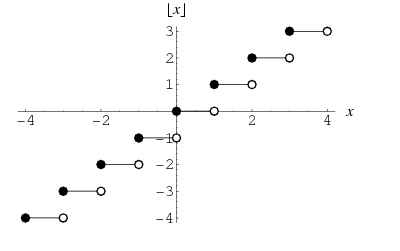
\includegraphics [scale=0.75] {floor.png} \end{center}
The floor function has one-sided limits (from the right) at integral values of $x$, but the limit at $x=2$, for example, does not exist, because those two one-sided limits are not the same.
\subsection*{example:  inverse}
Consider the function $f(x) = 1/x$.  This function is undefined at $x=0$ since division by zero is not defined.  As $x$ gets close to zero from the right, $1/x$ takes on larger and larger positive values.

Some people will say that limits can have infinite values.  In the case of $f(x) = 1/x$, informally, we accept that the limit as $x \rightarrow 0+$ exists and has the value $\infty$.  Speaking more formally, we might say that the function "diverges" or "grows without bound".

In any case since for $f(x) = 1/x$
\[ \lim_{x \rightarrow 0+} \ne \lim_{x \rightarrow 0-} \]
so the limit as $x \rightarrow 0$ does not exist (abbreviated D.N.E.).

\subsection*{example:  sine of 1/x}
The trigonometric functions sine and cosine are, of course, periodic.  For any value of $\theta$
\[ \sin \theta = \sin ( \theta \pm 2 \pi) \]
The maximum values of the sine function (for $\theta > 0$) occur at
\[ \theta = \frac{\pi}{2},  \frac{5\pi}{2}, \frac{9\pi}{2}, \frac{13\pi}{2} \dots \]
The corresponding maximum values of $\theta = 1/x$ occur at
\[ x = \frac{2}{\pi}, \frac{2}{5 \pi}, \frac{2}{9 \pi}, \frac{2}{13 \pi} \dots \]
The corresponding decimal values are approximately
\[ x = 0.6366, 0.1273, 0.0707, 0.0490 \]
As $\pi/2 + 2k\pi$ gets larger, the corresponding values for the inverse get smaller, and more closely spaced together.

Now, $1/x$ grows without bound as $x \rightarrow 0$.  This means that there is an infinite number of places where the value of the function $\sin(1/x)$ is equal to $1$ and indeed, takes on all possible values in its range $[-1,1]$, and this occurs more and more rapidly as $x \rightarrow 0$.

In short, the value oscillates and does so more extremely the closer $x \rightarrow 0$.
\begin{center} 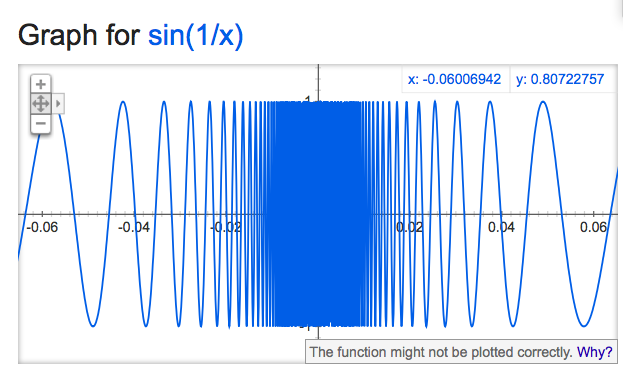
\includegraphics [scale=0.4] {sinxinverse.png} \end{center}
The limit as $x \Rightarrow 0$ D.N.E.

\end{document}  